\maketitle
\tableofcontents
\newpage

\section{Theorie}
Ziel des Versuches ist es, gekoppelte Schwingkreise im Hinblick auf Energietausch
mittels Schwebung und auf ihre Fundamentalschwingungen zu untersuchen.
Die gekoppelten Schaltkreise bestehen aus der Induktivität
$L$ und der Kapazität $C$. Die Kopplung besteht aus einem Kopplungskondensator
$C_{\symup{K}}$.
\begin{figure}
  \centering
  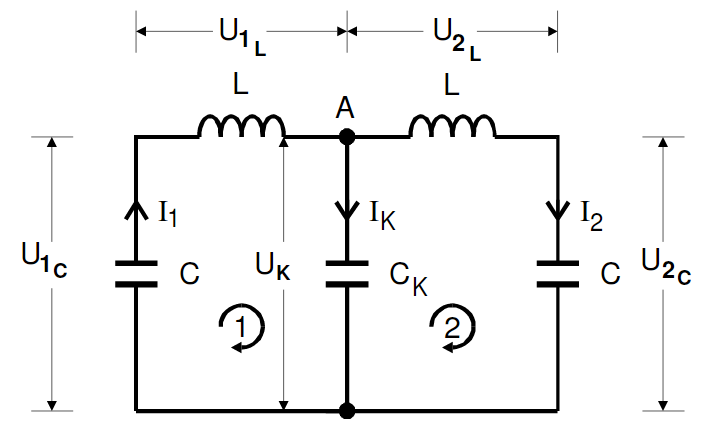
\includegraphics[scale=0.4]{theorie.png}
  \caption{Schaltbild zweier gekoppelter Schwingkreise \cite{anleitung}.}
  \label{fig:1}
\end{figure}
Aus Abbildung \ref{fig:1} lässt sich nun mithilfe der Kirchhoffschen Knoten-
und Maschenregel zwei Schwingungsgleichungen aufstellen
\begin{align}
    L\ddot{I}_1 + \frac{1}{C} \, I_1 + \frac{1}{C_{\symup{K}}} \left(I_1 - I_2\right) &= 0
    \label{eqn:1} \\
    L\ddot{I}_2 + \frac{1}{C} \, I_2 - \frac{1}{C_{\symup{K}}} \left(I_1 - I_2\right) &= 0 \, .
    \label{eqn:2}
\end{align}
Diese Differentialgleichungen sind voneinander abhängig und lassen sich deswegen
nicht ohne weiteres lösen. Durch Subtraktion von \eqref{eqn:1} und \eqref{eqn:2} erhält man
\begin{align}
    L \,  \frac{\symup d^2}{\symup d t^2} \left(I_1 + I_2 \right) + \frac{1}{C} \left(I_1 + I_2 \right) &= 0
    \label{eqn:3} \\
    L \,  \frac{\symup d^2}{\symup d t^2} \left(I_1 - I_2 \right) + \left(\frac{1}{C} + \frac{2}{C_{\symup{K}}} \right)
    \left(I_1 - I_2 \right) &= 0 \, .
    \label{eqn:4}
\end{align}
Damit lassen sich \eqref{eqn:3} und \eqref{eqn:4} unabhängig voneinander lösen; Die
Lösung von \eqref{eqn:3} ist hierbei eine harmonische Schwingung mit der Schwingungsfrequenz
\begin{equation}
    \nu_+ = \frac{1}{2\pi \sqrt{LC}} \, .
     \label{eqn:5}
\end{equation}
Diese Schwingung wird als gleichphasig bezeichnet. Diese wird dadurch ausgezeichnet,
dass beide Schwingkreise so schwingen, als wäre keine Kopplung vorhanden. Wenn man zwei
durch eine Feder gekoppelte Fadenpendel in die gleiche Richtung gleich weit auslenkt,
dann wird die Feder weder gestaucht noch gestreckt, sie verharrt in ihrem unausgelenktem
Zustand. Genauso verhält es sich mit zwei Schwingkreisen, die mit gleicher Amplitude und
Phase anfangen zu oszillieren.

Die Lösung von \eqref{eqn:4} hat die Schwingungsfrequenz
\begin{equation}
  \nu_- = \frac{1}{2\pi \sqrt{L \left(\frac{1}{C} + \frac{2}{C_{\symup{K}}} \right)^{-1}}} \, .
  \label{eqn:6}
\end{equation}
Diese Art der Schwingung wird als gegenphasig bezeichnet. Die Oszillation beginnt
mit gleicher Amplitude, aber entgegengesetzter Phase. Offensichtlich gilt
\begin{equation*}
    \nu_- > \nu_+ \, .
\end{equation*}
$\nu_+$ und $\nu_-$ sind die Frequenzen zu den Fundamentalschwingungen des gekoppelten Systems.

Ein weiteres interessantes Phänomen ergibt sich, wenn nur einer der beiden Schwingkreise
zum Zeitpunkt $t = 0$ einen Strom ungleich von 0 hat (hier Schwingkreis 1). Zu diesem
Zweck bildet man aus den Lösungen von \eqref{eqn:3} und \eqref{eqn:4} durch Umformungen
Ausdrücke für $I_1$ und $I_2$ (siehe Abbildung \ref{fig:1})
\begin{align}
    I_1(t) &= \frac{1}{2} \left(I_{1_0} + I_{2_0} \right) + \symup{cos} \left(2\pi v_+ t \right)
    + \frac{1}{2} \left(I_{1_0} - I_{2_0} \right) + \symup{cos} \left(2\pi v_- t \right)
    \label{eqn:7} \\
    I_2(t) &= \frac{1}{2} \left(I_{1_0} + I_{2_0} \right) + \symup{cos} \left(2\pi v_+ t \right)
    - \frac{1}{2} \left(I_{1_0} - I_{2_0} \right) + \symup{cos} \left(2\pi v_- t \right) \, .
    \label{eqn:8}
\end{align}
Falls man nun den oben beschriebenen Ansatz einsetzt und mit cos-Identitäten umformt,
erhält man aus \eqref{eqn:7} und \eqref{eqn:8}
\begin{align}
    I_1(t) &= I_{1_0} \symup{cos}\left(\frac{1}{2} \left(\omega_+ + \omega_- \right)t \right)
    \symup{cos}\left(\frac{1}{2} \left(\omega_+ - \omega_- \right)t \right)
    \label{eqn:9} \\
    I_2(t) &= I_{1_0} \symup{sin}\left(\frac{1}{2} \left(\omega_+ + \omega_- \right)t \right)
    \symup{sin}\left(\frac{1}{2} \left(\omega_+ - \omega_- \right)t \right) \, .
    \label{eqn:10}
\end{align}
Wenn man annimmt, dass $C_{\symup K} >> C$ gilt, dann folgt
\begin{align*}
    \frac{1}{2} \left(\omega_+ + \omega_- \right) &\approx \omega_+ \\
    \omega_- - \, \omega_+ &<< \omega_+ \, .
\end{align*}
Mit diesen Annahmen lässt sich aus \eqref{eqn:9} und \eqref{eqn:10} ablesen,
dass die Amplitude der ersten Schwingung genau dann ein Maximum hat,
wenn die Amplitude der zweiten Schwingung gleich 0 ist. Im Verlauf der Zeit
wird $I_2$ größer und $I_1$ kleiner, bis die Ausgangslage umgekehrt wurde.
\begin{figure}
  \centering
  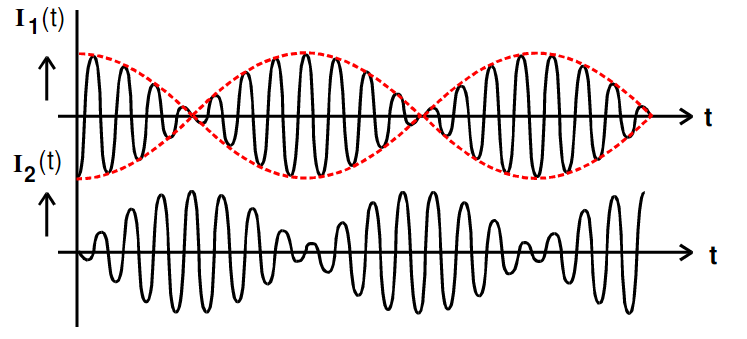
\includegraphics[scale=0.4]{schwebung.png}
  \caption{Amplitudenverlauf zweier Schwingungen, wenn eine Schwebung eintritt.}
  \label{fig:2}
\end{figure}
Diese Art der Schwingung, wie in Abbildung \ref{fig:2} zu sehen, nennt man Schwebung.
Die Frequenz $\nu_- - \, \nu_+$, mit der die Gesamtenergie des Systems zwischen
den Schwingkreisen oszilliert, wird als Schwebungsfrequenz bezeichnet.

\section{Durchführung}
Die Bauteilwerte lauten wie folgt:
\begin{align*}
  L &= \SI{23.954}{\milli\henry} \\
  C &= \SI{0.7932}{\nano\farad} \\
  C_{\symup{sp}} &= \SI{0.028}{\nano\farad}.
\end{align*}
$C_{\symup{sp}}$ gibt dabei die Kapazität der Spule an.

\subsection{Versuchsaufbau}
\label{sec:versuchsaufbau}
\begin{figure}
  \centering
  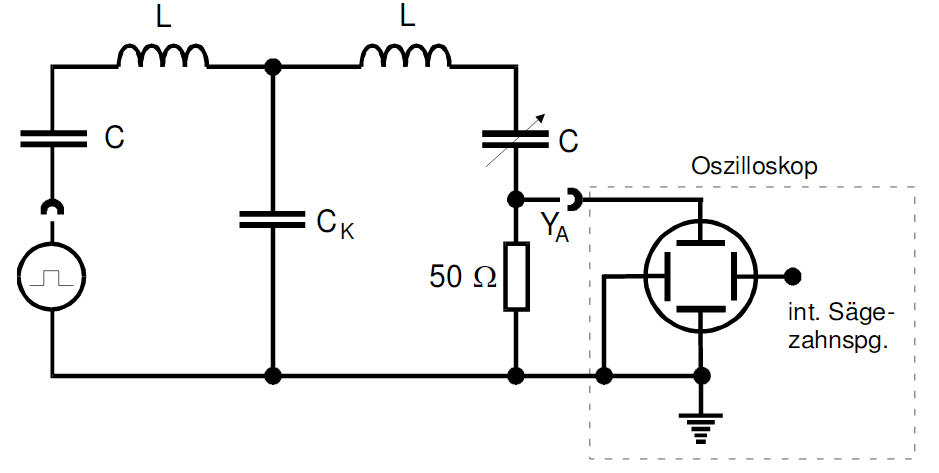
\includegraphics[scale=0.4]{aufbau.png}
  \caption{Schaltskizze zur Untersuchung des Schwebungsphänomens und,
  mit leichten Abwandlungen, zur Ermittlung der Fundamentalschwingungen.}
  \label{fig:3}
\end{figure}
Mit einer Rechteckspannung wird der linke $LC$ - Schwingkreis in Abbildung \ref{fig:3}
angeregt. Über den Kopplungskondensator $C_{\symup{K}}$ gelangt die Schwingung in den
rechten Teil des gekoppelten Schwingkreises (mit einem kapazitiv verstellbaren Kondensator),
wo über den einen ohmschen Widerstand ein Oszilloskop die Schwebung sichtbar macht.

Um die Fundamentalschwingungen zu bestimmen, wird in Abbildung \ref{fig:3} die Rechteck- durch
eine Sinusspannung ersetzt und jene ebenfalls auf das Oszilloskop gegeben.

\subsection{Versuchsdurchführung}
\begin{figure}
  \centering
  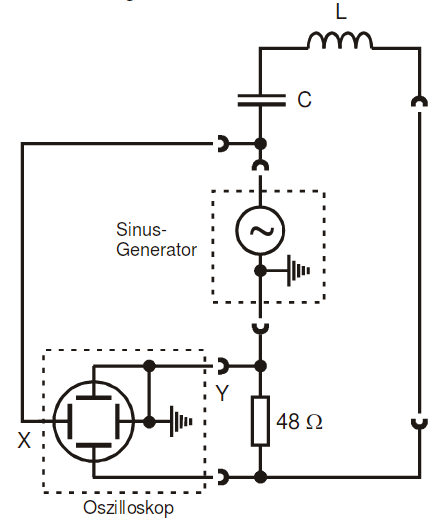
\includegraphics[scale=0.4]{justierung.png}
  \caption{Schaltskizze zur Justierung des einstellbaren Kondensators im rechten
  Schwingkreis in Abbildung \ref{fig:3}.}
  \label{fig:4}
\end{figure}
Zuerst wird mithilfe der Schaltung aus Abbildung \ref{fig:4} der rechte Schwingkreis unter Zuhilfenahme des einstellbare Kondensator
aus Kapitel \ref{sec:versuchsaufbau} auf die Resonanzfrequenz des anderen Schwingkreises eingestellt.
Zu diesem Zweck wird mit Hilfe von Lissajous-Figuren die Frequenz gesucht, bei der
die Phase zwischen Generatorspannung und Schwingkreisstrom im linken Schwingkreis gleich $\frac{\pi}{2}$ ist.
Alsdann wird der Vorgang für den rechten Schwingkreis wiederholt, diesmal wird jedoch
die eben bestimmte Resonanzfrequenz durch den verstellbaren Kodensator eingestellt.

Um das Verhältnis zwischen Schwingungs- und Schwebungsfrequenz zu bestimmen, wird
für alle möglichen Kopplungskondensatoren $2 \le C_{\symup{K}} \le \SI{12}{\nano \farad}$
die Anzahl der Schwingungsmaxima innerhalb einer Schwebungsperiode gezählt. Dies
lässt sich über das Oszilloskop aus \ref{sec:versuchsaufbau} bewerkstelligen.

Weiterhin sollen die Fundamentalschwingungen $\nu_+$ und $\nu_-$ bestimmt werden.
Wie in Kapitel \ref{sec:versuchsaufbau} beschrieben werden Sinusspannung und Schwingkreisstrom
im Oszilloskop gegeneinander aufgetragen und mithilfe von Lissajou-Figuren die Frequenzen
gesucht, bei denen die Phase 0 ($\nu_+$, da $\nu_+ < \nu_-$) bzw. $\pi$ ($\nu_-$) ist.
Dabei werden erneut alle möglichen Kopplungskondensatoren $2 \le C_{\symup{K}} \le \SI{12}{\nano \farad}$
nacheinander eingeschaltet.

Eine andere Methode, um die Fundamentalschwingungen zu bestimmen, ist der sogenannte Sweep.
Dabei wird, in diesem Fall, in einer Sekunde das Frequenzspektrum von einer beliebigen
Anfangs- bis zu einer beliebigen Endfrequenz auf einem Oszilloskop dargestellt. Zu sehen
sind dann (neben zwei kleinen Peaks, die Anfangs- und Endzeitpunkt darstellen) zwei
große Peaks, die die Frequenzen $\nu_+$ und $\nu_-$ (in der Reihenfolge) darstellen.
Dies wird erneut in Abhängigkeit von $C_{\symup{K}}$ gemessen.
\section{Auswertung}
Die Fehler wurden in "python" mithilfe des Paketes "uncertainties"\footnote{Versionen: python 3.5.1, uncertainties 3.0.1} bestimmt.
\subsection{Bestimmen der Resonanzfrequenz des festen und Jusatage des regelbaren Schwingkreises}
Die gemessene Resonanzfrequenz des festen Schwingkreises beträgt \SI{35.65}{\kilo\hertz}
bei einem geschätzten Fehler von \SI{20}{\hertz}. Nach \eqref{eqn:5}
folgt für die theoretische Resonanzfrequenz ein Wert von \SI{36.51}{\kilo\hertz}. Die relative Abweichung
zwischen Theorie und Experiment beträgt \SI{2.36}{\percent}, liegt also in einem vertretbar
kleinen Bereich, aber dennoch außerhalb des angenommenen Fehlers.
Der regelbare Schwingkreis wird entsprechend so eingestellt, dass er
dieselbe Resonanzfrequenz hat.
\subsection{Messung der Fundamentalfrequenzen anhand der Phasenverschiebung zwischen Erreger- und Schwingkreisspannung}
\label{aus:1}
\begin{table}
  \centering
  \begin{tabular}{c c c c}
    \toprule
  $C_{\symup{k}}/\si{\nano\farad}$ & $ \frac{f_{\symup{Schwebung}}}{f_{\symup{Schwingung}}}$ &
  $\nu_+/\si{\kilo\hertz}$ & $\nu_-/\si{\kilo\hertz}$\\
    \midrule
    2.19 & 8 & 35.71 & 46.51 \\
    2.86 & 8 & 35.71 & 44.44 \\
    4.74 & 14 & 35.71 & 41.67 \\
    6.86 & 20 & 35.71 & 40.00 \\
    8.18 & 22 & 35.71 & 39.22 \\
    9.99 & 26 & 35.71 & 38.46 \\
    12 & 32 & 35.71 & 37.74 \\
    \bottomrule
  \end{tabular}
  \caption{Messwerte für die Fundamentalfrequenzen sowie das Verhältnis zwischen
  Schwingungs uns Schwebungsfrequenz, welches für eine vollständige Periode
  der Einhüllenden gemessen wurde. Die $C_{\symup{k}}$ werden in den Rechnungen
   mit dem auf der Apperatur angegebenen Fehler von $\pm \, \SI{0.3}{\percent}$ behandelt, die
   Frequenzen mit einem geschätzten Fehler von $\pm \, \SI{20}{\hertz}$ und die Anzahl
   der Maxima mit $\pm \, 1$.}
   \label{tab:1}
\end{table}
Die Messwerte sind in Tabelle \ref{tab:1} dargestellt.
Nach \eqref{eqn:5} mit
\begin{equation}
   C_{\symup{ges}} = C + C_{\symup{sp}}
\end{equation}
folgt für die von der Kapazität des Kopplungskondensators unabhängige,
theoretische, gleichphasige Schwingung ein Wert von \SI{35.89}{\kilo\hertz}. Dieser Wert liegt nicht
in der angenommenen Fehlertoleranz des Messwertes,
die relative Abweichung zwischen Theorie und Experiment beträgt dennoch lediglich \SI{0.49}{\percent}.\\
\\
Für die Fundamentalfrequenz der gegenphasigen Schwingung folgen nach \eqref{eqn:6} mit
\begin{equation}
  C_{\symup{ges}} = C_{\symup{sp}} + \left( \frac{1}{C} + \frac{2}{C_{\symup{k}}} \right)^{-1}
\end{equation}
die in Tabelle \ref{tab:2} dargestellten
Werte für die einzelnen Kapazitäten des Kopplungskondensators.
Ebenfalls in dieser Tabelle sind die relativen Abweichungen zwischen den Theorie- und
Messwerten eingetragen. Die relativen Fehler sind wieder extrem gering. Die Werte für $C_{\symup{k}} = \SI{2.19}{\nano\farad}$
liegen desweiteren im Rahmen ihrer gegenseitigen Messungenauigkeit, betrachtet man die
Überscheidung beider Fehlerintervalle.
\begin{table}
  \centering
  \begin{tabular}{c c c c}
    \toprule
  $C_{\symup{k}}/\si{\nano\farad}$ & $\nu_-/\si{\kilo\hertz}$ & $\nu_{- \, , \symup{rechnerisch}}/\si{\kilo\hertz}$
  & relative Abweichung/\si{\percent}\\
    \midrule
    2.19 & 46.51 & \num{46.55(3)} & 0.09 \\
    2.86 & 44.44 & \num{44.33(2)} & 0.26 \\
    4.74 & 41.67 & \num{41.22(2)} & 1.07 \\
    6.86 & 40.00 & \num{39.66(1)} & 0.84 \\
    8.18 & 39.22 & \num{39.08(1)} & 0.35 \\
    9.99 & 38.46 & \num{38.52(1)} & 0.17 \\
    12.00 & 37.74 & \num{38.10(1)} & 0.95 \\
    \bottomrule
  \end{tabular}
  \caption{Werte für die experimentell und theoretisch bestimmten gegenphasigen
  Fundamentalfrequenzen sowie der relative Fehler zwischen diesen Werten. Alle
  gemessenen Frequenzen werden mit einem Fehler von $\pm \, \SI{20}{\hertz}$ angenommen.}
   \label{tab:2}
\end{table}
Aus:
\begin{equation}
  \frac{f_{\symup{Schwebung}}}{f_{\symup{Schwingung}}} = n_{\symup{Maxima}} =
  \frac{(\nu_+ + \nu_-)}{(\nu_- - \nu_+)}
\end{equation}
folgen mit den oben theoretisch berechneten Werten die in Tabelle \ref{tab:3} dargestellten
Werte für eine vollständige Schwingung der Einhüllenden. Wieder zeigen sich geringe relative Abweichungen.
Für einen Teil der Werte liegen theoretische und experimentelle Werte im Bereich der angenommenen
Messungenauigkeit.
\begin{table}
  \centering
  \begin{tabular}{c c c c}
    \toprule
  $C_{\symup{k}}/\si{\nano\farad}$ & $n_{\symup{Max.}}$ & $n_{\symup{Max., theo.}}$
  & relative Abweichung/\si{\percent}\\
    \midrule
    2.19 & 8 & \num{7.73(2)} & 3.51 \\
    2.86 & 8 & \num{9.50(2)} & 15.81 \\
    4.74 & 14 & \num{14.45(4)} & 3.08 \\
    6.86 & 20 & \num{20.00(5)} & 0.01 \\
    8.18 & 22 & \num{23.45(7)} & 6.19 \\
    9.99 & 26 & \num{28.18(8)} & 7.75 \\
    12.00 & 32 & \num{33.44(9)} & 4.30 \\
    \bottomrule
  \end{tabular}
  \caption{Werte für die experimentell und theoretisch bestimmten Verhältnisse
  zwischen Schwingungs- und Schwebungsfrequenz sowie der relative Fehler zwischen diesen Werten.
  Die experimentellen Werte werden dabei mit einem Fehler von $\pm \, \num{1}$ angenommen.}
   \label{tab:3}
\end{table}
\subsection{Messung der Fundamentalfrequenzen durch einen Frequenz-Sweep}
\begin{table}
  \centering
  \begin{tabular}{c c c c c}
    \toprule
  $C_{\symup{k}}/\si{\nano\farad}$ & $t / \si{\milli\second}$ & $\nu_-/\si{\kilo\hertz}$ &
  $\nu_{- \, , \symup{rechnerisch}}/\si{\kilo\hertz}$ & relative Abweichung/\si{\percent}\\
    \midrule
    0.997 & 712 & \num{54.88(49)} & \num{56.26(5)} & 2.50 \\
    2.190 & 528 & \num{45.88(49)} & \num{46.55(3)} & 1.45 \\
    2.860 & 484 & \num{43.73(49)} & \num{44.33(2)} & 1.36 \\
    4.740 & 416 & \num{40.41(49)} & \num{41.22(1)} & 2.02 \\
    6.860 & 384 & \num{38.84(49)} & \num{39.66(1)} & 2.11 \\
    8.180 & 372 & \num{38.25(49)} & \num{39.08(1)} & 2.16 \\
    9.990 & 360 & \num{37.67(49)} & \num{38.52(1)} & 2.28 \\
    12.000 & 344.00 & \num{36.89(49)} & \num{38.10(1)} & 3.29 \\
    \bottomrule
  \end{tabular}
  \caption{Werte für die experimentell und theoretisch bestimmten Fundamentalfreuqenzen
  $\nu_-$ sowie den relative Fehler zwischen diesen Werten. Die Zeiten werden mit einem
  angenommen Fehler von $\pm \, \SI{10}{\milli\second}$ behandelt.}
   \label{tab:4}
\end{table}
Mit der in der Durchführung beschriebenen Methode folgt ein Frequenzsspektrum:
\begin{equation}
  f(t) = f_{\symup{Start}} + (f_{\symup{Ende}} - f_{\symup{Start}}) \cdot \frac{t}{t_{\symup{Sweep}}}
  \label{eq:1}
\end{equation}
mit $ 0 \le t \le t_{\symup{Sweep}}$. $f_{\symup{Ende}}$ bezeichnet die Startfrequenz,
$f_{\symup{Start}}$ die Endfrequenz und $t_{\symup{sweep}}$ die Sweep-Dauer von einer Sekunde.
Für den bei $t=\SI{308}{\milli\second}$ gemessenen $\nu_+$-Peak folgt daraus eine
Frequenz von \SI{35.12(49)}{\kilo\hertz}. Im Vergleich mit dem in \ref{aus:1} bestimmten,
rechnerischen Wert von $\nu_+$ folgt eine relative Abweichung von \SI{2.12}{\percent}.
$\nu_+$ wurde acht mal gemessen, ohne dass sich der Wert ändert.
Der Wert liegt nicht im Bereich der angenommenen Messungenauigkeit von $\pm \, \SI{10}{\milli\second}$.\\
\\
In Tabelle \ref{tab:4} sind die gemessenen Zeiten zwischen Startpunkt und dem $\nu_-$-Peak,
die damit aus \eqref{eq:1} berechneten Frequenzen sowie die relativen Abweichungen zu den ebenfalls aufgeführten
theoretischen Frequenzen angegeben. Keiner der Werte liegt im Bereich der Messungnauigkeit.
Die relativen Fehler sind jedoch auch hier gering.
\section{Diskussion}
\begin{figure}
  \centering
  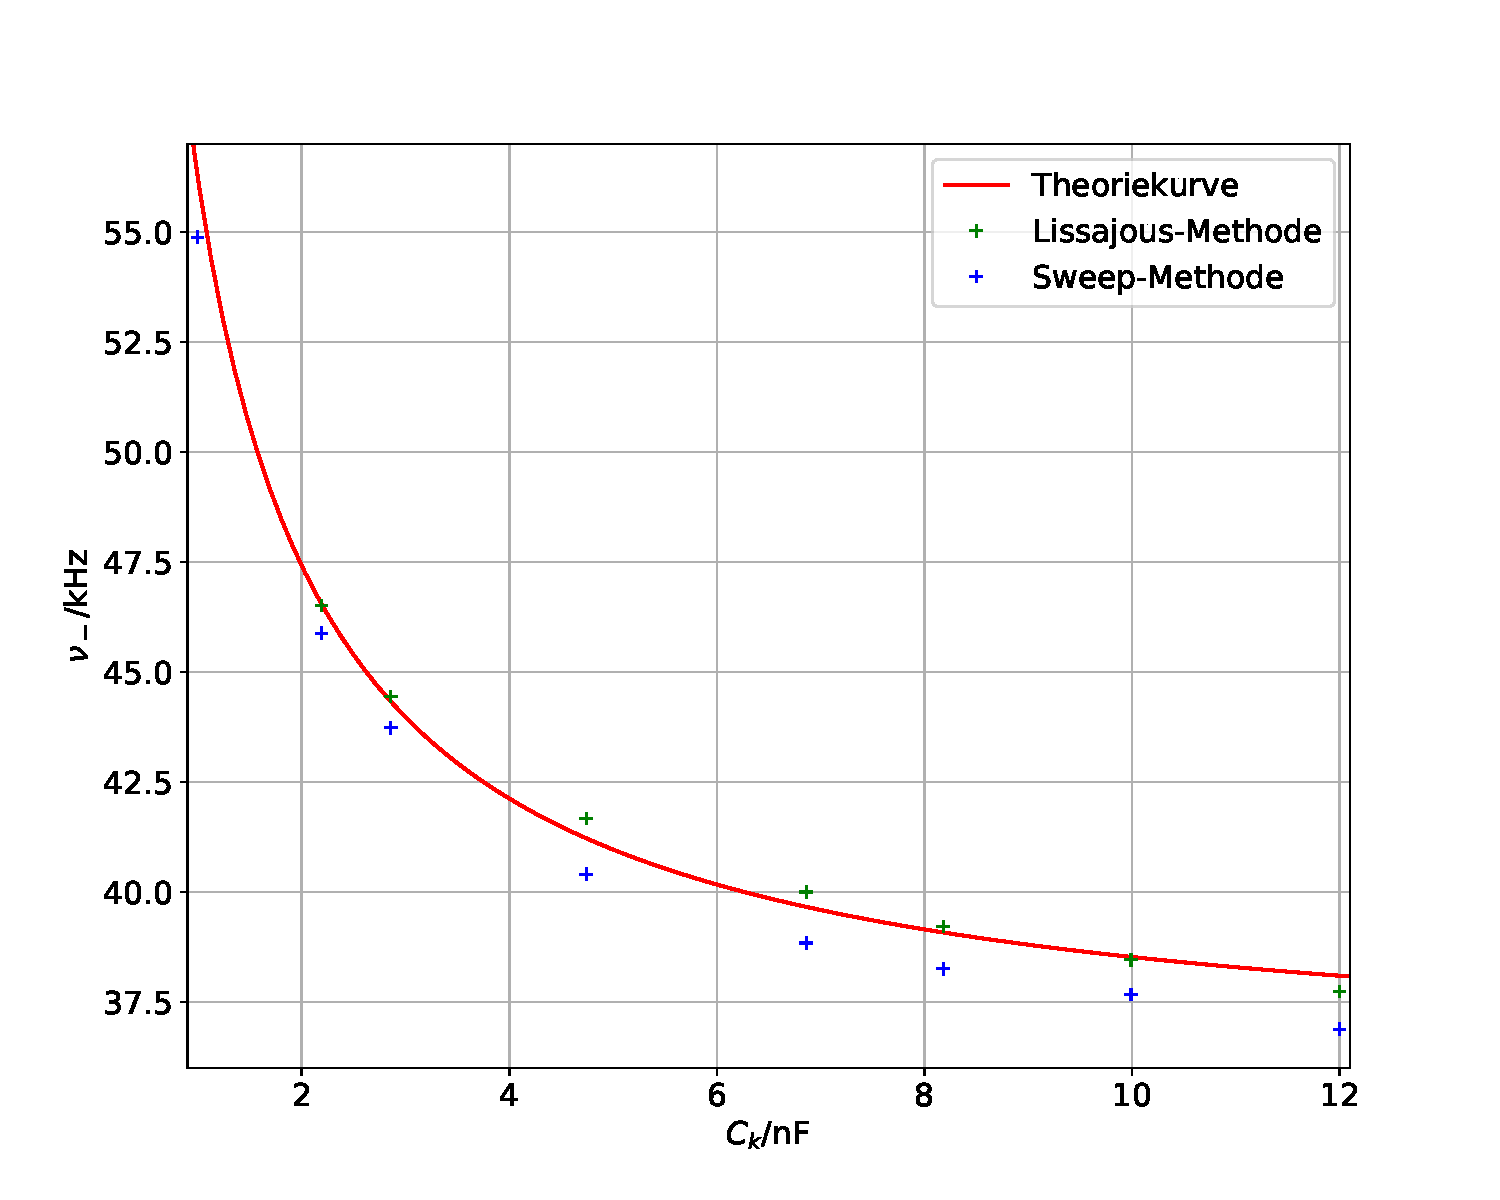
\includegraphics[scale=0.6]{Methoden.pdf}
  \caption{Aus den einzelnen Methoden sowie rechnerisch erhaltene Werte für $\nu_-$ in
  Abhängigkeit der Kapazität des Kopplungskondensators.}
  \label{abb:1}
\end{figure}
In Abbildung \ref{abb:1} sind die aus den einzelnen Methoden erhaltenen Werte dargestellt.
Es zeigt sich, dass die über Lissajous-Figuren bestimmten Frequenzen näher an den Theoriewerten
sind als die aus der Sweep-Methode. Dies lässt sich durch die Art der Messwertaufnahme erklären.
Während Lissajous-Figuren deutlich und ohne große Abweichungen zu erkennen sind,
begünstigt das Ablesen eines Peaks durch den Coursor systematische Fehler. Es kann nicht
mit ausreichender Sicherheit festgestellt werden, ob der exakt richtige Punkt getroffen wurde.
Dennoch sind die relativen Abweichungen bei beiden Methoden im niedrigen, einstelligen Prozentbereich.
Sie stellen also beide eine gute Möglichkeit dar, die Fundamentalfrequenzen eines Schwingkreises
zu bestimmen. Dies fällt auch beim Vergleich der ebenfalls bestimmten $\nu_+$-Frequenzen auf.
Auch die Zählung der Maxima innerhalb einer Schwebungsperiode zeigt, dass
Theorie und Messergebnis bei diesem Versuch nahe beieinander liegen und verifiziert daher die
Ergebnisse aus der Bestimmung der Fundamentalfreuqenzen. Die vergleichsweise hohen Abweichungen
lassen sich durch die im hohen einstelligen bis niedrigen zweistelligen Bereich liegenden Werte
erklären. Dort sorgen bereits geringe Unterschiede zwischen den Werten
für relativ hohe prozentuale Abweichungen.\\
\\
Zur Verbesserung der Messgenauigkeit bieten sich präzisere Geräte an. Ansonsten liefern die
Messungen aber für den betriebenen Aufwand und die zur Verfügung stehenden Geräte sehr gute
Ergebnisse.
\newpage
\nocite{*}
\printbibliography
